% !TeX root = ../bnuthesis-example.tex

\counterwithin{figure}{chapter}

\chapter{绪论}

本章从介绍强场物理、真空对产生、研究现状等方面阐述强场下真空中产生正反粒子的研究背景和研究意义。最后,我们将介绍本论文的主要研究内容。

\section{强场物理简介}

自20世纪60年代第一台激光器诞生 \cite{1960jiguang}以来,它极大地推动了科技进步,彻底改变了人类的生活,现已成为科学研究、医学治疗、工业生产和国防等领域中不可或缺的重要工具。随着激光技术的发展,激光聚焦强度得到了极大地提高,强场物理、激光等离子体物理、核聚变、超快和阿秒科学、新型粒子加速器技术等领域都取得了重大突破。随着基于啁啾脉冲放大技术(chirped pulse amplification, CPA)的超短、高功率激光器的发展,强场物理蓬勃发展\cite{2019GM}。

\begin{figure}
  \centering
  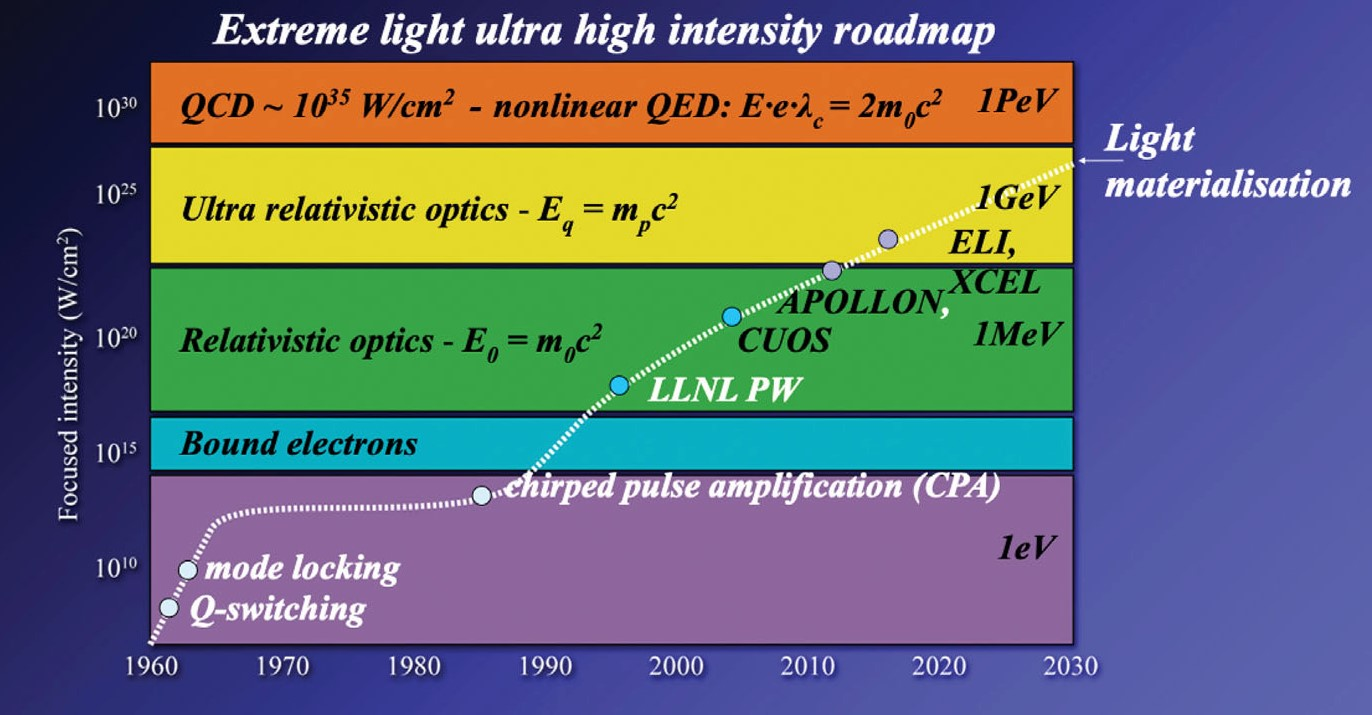
\includegraphics[width=0.8\linewidth]{figures/fig/fig1.1.jpg}
  \caption{激光发展史。}
  \label{tu1}
\end{figure}

如图~\ref{tu1}所示是激光发展史。激光强度小于$ 10^{14}~\mathrm{W/cm^{2}}$,此时激光所提供的电场强度不能够直接电离出原子中的束缚电子,此阶段强场物理研究激光与原子分子相互作用。激光强度处于$10^{14}~\mathrm{W/cm^{2}}\backsim 10^{18}~\mathrm{W/cm^{2}} $,激光的电场可以直接使得原子发生电离,形成等离子体,此阶段强场物理主要研究激光与等离子体相互作用。激光强度大于 $ 10^{18}~\mathrm{W/cm^{2}}$,使得我们对光与物质相互作用的研究进入了相对论非线性区域与非相对论性区域相比,激光场更有效地移动物质,粒子运动的高度非线性导致了很多新奇的物理现象,例如强激光场的Compton散射\cite{2018Compton},激光尾场加速\cite{2010wei},相对论自聚焦\cite{1974zi,1995zi}。

目前,激光强度达到了$ 10^{23}~\mathrm{W/cm^{2}}$的量级 \cite{2021jiguang},为了进一步提高激光强度,各地区正在建设的输出功率达到或超过10PW超高功率激光设施,如中国的极端光物理线站(Station of Extreme Light,SEL)\cite{2018SEL},法国的Apollon\cite{2015Apollon},欧盟的ELI(Extreme Light Infrastructure)\cite{2018ELI},美国的EP-OPAL(OMEGA EP-coupled Optical Parametric Amplifier Lines)\cite{2019OP},计划把激光强度达到$10^{23}~\mathrm{W/cm^{2}}\backsim 10^{24}~\mathrm{W/cm^{2}} $。对于强场量子电动力学(strong field quantum electrodynamics,SFQED)的探索,迫切需要激光强度超过$ 10^{23}~\mathrm{W/cm^{2}}$的超高功率激光器\cite{2019jiguan,2020jiguan}。在这个强度水平下,SFQED现象变得可观察;通过非线性康普顿散射(nonlinear Compton scattering, NCS)可以发射出超强的伽马射线,通过非线性布莱特-惠勒(Breit–Wheeler process,BW)过程可以产生电子-正电子对\cite{2006dzheng,2012zheng,2018zheng,2022zheng}。

\section{真空对产生}

根据Heisenberg的不确定性原理,我们知道在能量和时间上满足$\delta E \cdotp \Delta t \ge \frac{\hbar}{2}$,$\hbar$是普朗克常数。真空在极短时间内会有非常大的能量变化,对应着正负虚粒子的产生和湮灭。这就是真空涨落,2015年康斯坦茨大学的科研人员们直接验证了真空涨落现象的存在\cite{2015f},见图\ref{tu3}。这就是常说的“真空不空”,我们可以把真空看作是具有一定折射率和吸收率的极化介质。对于比较弱的外场,真空的结构非常稳定的,量子涨落所产生的虚粒子又很快湮灭掉而无法转换成实粒子。但在非常强的外场下,量子涨落所产生的虚粒子被强外场所拉开而不再发生湮灭,从而演化得到实粒子对,见图\ref{tu4}。在真空中能够产生一对正负电子对的临界电场可以通过在该电场下电场力把正负电子对拉开一个Compton波长的距离所做的功和电子的静止能量相等这一关系即$E_{\mathrm{cr}}=m^2c^{3} / e \hbar$估算出来,其中$m$是电子的静止质量,$c$是光速,$e$是电子电荷,

\begin{figure}
  \centering
  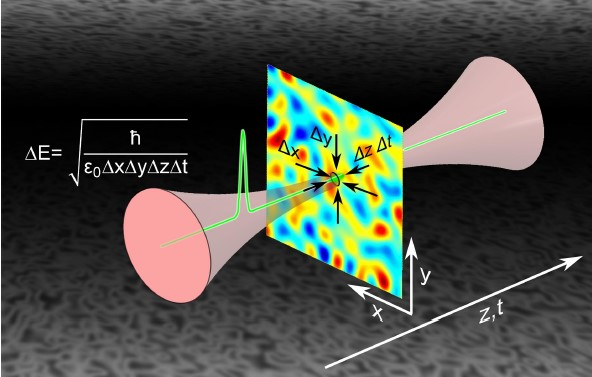
\includegraphics[width=0.8\linewidth]{figures/fig/fig1.3.jpg}
  \caption{真空涨落示意图}
  \label{tu3}
\end{figure}
\begin{figure}
  \centering
  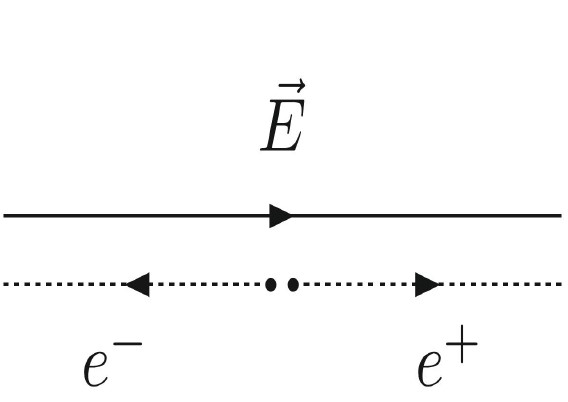
\includegraphics[width=0.8\linewidth]{figures/fig/fig1.4.jpg}
  \caption{强外场下真空产生正负电子对示意图}
  \label{tu4}
\end{figure}

随着激光强度的不断提高,光转化成物质是SFQED中的研究热点话题之一。由于需要对产生过程需要满足动量守恒和能量守恒,所以单个的平面波是不可能产生正负电子对。因此我们想要实现对产生,还需要在场中增加其他能量源来引发这个过程。有三种方法来实现对产生,见图~\ref{tu2}。(图(a)和(b)里的黑色实线代表Volkov正负能态,(b)中叉号顶点代表库仑场,(c)中的双线表示在驻波场中的电子传播子。如图~\ref{tu2}(a)所示是高能光子与强激光场中传播,高能光子与激光相互作用产生正负电子对。如图~\ref{tu2}(b)所示是激光在库仑场中传播,激光与原子核的库仑场相互作用产生正负电子对。如图~\ref{tu2}(c)所示,是利用两束激光对撞形成的驻波场来促进正负电子对的产生。

以上三种对产生机制,物理学家们已经在实验室实现了前两种。1996年,Bula等人使用斯坦福直线加速器(SLAC)产生的$46.6\mathrm{GeV}$的电子束和光子能量为$2.4\mathrm{eV}$,激光强度为$1.3 \times10^{18}~\mathrm{W/cm^{2}}$的强激光对撞验证了第一种正负电子对产生机制\cite{1996BW}。在这次电子与激光对撞实验中,科研人员利用多普勒效应,提高了在粒子静止系重点激光强度和激光频率,有效地促进了对产生过程。在该实验过程中,电子与激光光子对撞,发生NCS过程($e^- + n \omega_0 \to \acute e^- + \omega$),即产生了高能$\gamma$光子,频率为$\omega$。然后高能$\gamma$光子再与激光光子发生多光子Breit-Wheeler过程($\omega + n \omega_0 \to e^+ e^-$)产生正负电子对。

2010年,Chen等人利用$10^{20}~\mathrm{W/cm^{2}}$强激光照射金靶,在金靶后探测到正电子束\cite{2010BH},实现了第二种正负电子对产生机制,在实验过程中激光光子和金原子核发生散射产生高能$\gamma$光子,然后高能$\gamma$光子和高Z核发生Bethe-Heitler过程($Z+n \omega_{0} \rightarrow Z+e^{+}+e^{-}$)产生正负电子对。前面两种方式利用多普顿效应促进激光强度和频率在粒子静止系提升,从而增强对产生。第三种方式利用两束激光场对撞形成的驻波场来产生正负电子对,无法利用上述的机制来促进对产生,这样就导致需要的电场强度非常高,因此尚未在实验室中得到第三种机制产生正负电子对,这也是研究人员们一直在攻克的难题。

在下文中,我们对第三种正负电子对形成的不同机制(Schwinger机制和多光子过程)进行简要概述。为了形象化地表达物理本质,我们使用了一个经典的描绘真空状态的图像:狄拉克海图像。尽管我们知道这个图像已经过时,且与现代量子场论知识不兼容,但在许多方面,它仍然作为一个经典并且便于理解的物理模型存在。

\begin{figure}
  \centering
  \includegraphics[width=0.8\linewidth]{figures/fig/fig1.2.pdf}
  \caption{对产生三种过程的费曼图}
  \label{tu2}
\end{figure}

\subsection{Schwinger机制}

在真空中产生正负电子对是量子电动力学(quantum electrodynamics ,QED)中最有趣理论之一。1928年,Dirac在理论上预言了反物质存在\cite{1928s},具体来说,他预测了正电子的存在。Anderson的实验验证了这一预言,确凿无疑地证明了正电子的存在\cite{1933s}。1931年,Sauter提出产生真空中正负电子对这一问题\cite{1931s}。1936年,Heisenberg和Euler采用了有效拉格朗日量方法对对产生问题进行了进一步完善\cite{1936s}。到了1951年,Schwinger对真空对产生现象有了完整的理论描述\cite{1951s},为了纪念Schwinger在的卓越贡献,因此人们把在强场下真空通过隧穿效应产生正负电子对的过程成为Schwinger机制或者Schwinger效应。

一般来说,基本的物理思想是将真空状态视为一种材料,具有明显分离的导带(正能连续态)和价带(狄拉克海)。这两个带之间的带隙被假定为粒子和相应的反粒子的静止质量;在我们研究的情况下,是电子和正电子的质量。在真空状态下,正能连续态中没有电子,然而狄拉克海完全充满了具有负能量的电子。由于所有可观察的粒子必须具有正能量,因此我们观察不到狄拉克海的物质,例如有一束能量强至$2m c^{2}$的光子将狄拉克之海中的一个负能量电子提升为一个具有正能量的电子,那么在狄拉克之海中就会留下一个洞。这个洞相当于狄拉克之海中的一个粒子,它同时具有负能量态电子的所有相反属性,即具有正能量和正电荷。因此粒子创造的问题可以归结为将粒子从狄拉克海带到连续态的问题。由于这些带中的每一个空穴都可以与一个反粒子关联,所以上述的想法也同样适用于反粒子。

为了阐明导致电子对产生的各种机制,我们需要对真空态施加强电场。外部强场会使能带发生变形,如图\ref{tu5}所示,深蓝色能带代表着狄拉克海,浅红色能带代表着连续态。能带间隙(白色部分)是真实粒子禁止区域。。因此,从狄拉克海中激发电子到导带的各种情况变得可能。如果施加电场的场强是$E_{\mathrm{cr}}$的数量级,能带会发生强烈的变形,使电子可以从一个能带简单地隧穿到另一个能带。这种现象被称为施温格效应。如图\ref{tu6}展示了这样一个隧穿过程的示意图,当系统受到强电场作用时,能带会发生变形,使电子(黑点)可以隧穿到连续态。

\begin{figure}
  \centering
  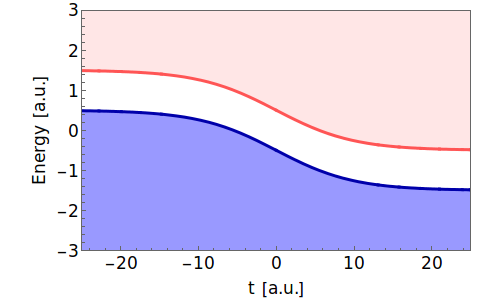
\includegraphics[width=0.8\linewidth]{figures/fig/fig1.5.png}
  \caption{强场下的能带图}
  \label{tu5}
\end{figure}

\begin{figure}
  \centering
  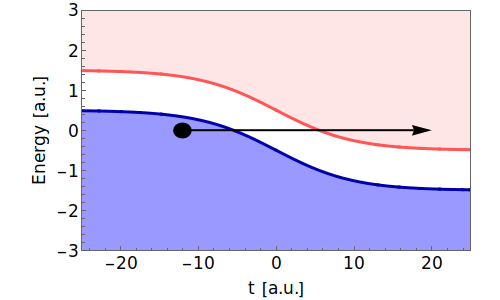
\includegraphics[width=0.8\linewidth]{figures/fig/fig1.6.png}
  \caption{施温格效应的图像描述}
  \label{tu6}
\end{figure}

下面我们来推导在Schwinger机制下的真空正负电子对的产生几率。从之前Sauter的工作中,在强电场下解狄拉克方程时,发现真空的正负能带在电场下会发生弯曲,对于足够大的电场强度,能级甚至可能发生交错。此时,根据量子隧道效应,负能带中的电子的将有一定概率隧道到正能带形成电子,同时在负能带中留下一个空穴,这个空洞就是电子的反物质-正电子的空穴理论。这就是量子力学中强场下真空生成正负电子对的物理图像。然后,可以从量子隧道的透射系数得到真空对生成的几率

\begin{equation}
    \mathcal{\Gamma}_{e^{-} e^{+}} \sim \exp \left(-\pi \frac{E_{\mathrm{cr}}}{|\mathbf{E}|}\right),
\end{equation}
其中,$E_{\mathrm{cr}}$为临界电场,$E$为外电场强度。

在Dunne的工作中\cite{2005L,2012L},对欧拉-海森堡拉格朗日量对理论物理的影响进行了回顾。欧拉-海森堡拉格朗日量通过非线性项扩展了麦克斯韦拉格朗日量,涵盖了在背景电磁场中产生的量子效应,表达式如下

\begin{equation}
 \mathcal L = \frac{e^2}{h c} \int_0^{\infty} \frac{d \eta}{\eta^3} e^{-\eta} \times \\
 { i\eta^2 {\mathbf{E} \cdot \mathbf{B}} 
 \frac{\cos {\frac{\eta}{E_0} \sqrt{\mathbf{E}^2 - \mathbf{B}^2 + 2 i{\mathbf{E} \cdot \mathbf{B}} }} +c.c}{\cos {\frac{\eta}{E_0} \sqrt{\mathbf{E}^2 - \mathbf{B}^2 + 2 i {\mathbf{E} \cdot \mathbf{B}} }} -c.c}
 + E_0^2 + \frac{\eta^2}{3} {\mathbf{B}^2 - \mathbf{E}^2} },
\end{equation}
其中,$ E_0 = \frac{m^2 c^3}{e \hbar} \approx 1.3 \ 10^{18} \ V/m$,$ E_0$首次在参考文献\cite{1931s}中确定,被定义成在真空在恒定电场下创造物质的临界场强。通过对弱场进行摄动展开拉格朗日量,可以获得对麦克斯韦拉格朗日量的主要量子修正

\begin{equation}
\mathcal{L}_{pert}  = \frac{\mathbf{E}^2 - \mathbf{B}^2}{2} + \frac{1}{90 \pi} \frac{\hbar c}{e^2} \frac{1}{E_0^2} { {\mathbf E^2 - \mathbf B^2}^2 + 7 {\mathbf{E} \cdot \mathbf B}^2}.
\end{equation}
值得注意的是,拉格朗日量完全是以洛伦兹不变量的形式构建的
\begin{equation}
\mathcal F = -\frac{1}{4} F^{\mu \nu} F_{\mu \nu} = \frac{1}{2} {\mathbf{E}^2 - \mathbf{B}^2} ,\qquad \mathcal G = -\frac{1}{4} F^{\mu \nu} \tilde F_{\mu \nu} = \mathbf{E} \cdot \mathbf{B}
\end{equation}
其中,第二项被临界场强$E_0$抑制。

在发展重整化方案并将其纳入量子电动力学以形成电磁力的完全协变表述的过程中,利用新技术进一步研究了对产生问题。将对产生过程视为适当时空的演化过程\cite{1951s}, Schwinger能够将物质的创造与恒定场的有效拉格朗日量联系起来
\begin{equation}
 \mathcal L = \frac{1}{2} E^2 - \frac{1}{8 \pi^2} \int_0^{\infty} \frac{ds}{s^3} \left ( {e E \ s \ \text{cot} {\left ( e E \ s \right ) } - 1 + \frac{1}{3} {\left ( e E \ s \right ) }^2}\right ). 
\end{equation}
它的虚部特别重要
\begin{equation}
    \text{Im} \ \mathcal L = \frac{\alpha^2}{2 \pi^2} E^2 \sum_{n=1}^{\infty} n^{-2} \exp {\frac{-n \pi m^2}{e E}}.
\end{equation}
以上描述了恒定电场中真空衰变速率。此外,这个求和的第一项给出了单个电子-正电子对的产生率:
\begin {equation} \label{NS}
 \dot N = \frac{\alpha^2}{2 \pi^2} E^2 \exp {\frac{- \pi m^2}{e E}}.
\end {equation} 

\subsection{多光子过程}

第二种机制是电子通过吸收高能光子而激发。在这种情况下,电子吸收了光子的能量,导致电子的净能量足够克服带隙(见图\ref{tu7}左);如果同时吸收了多个光子,我们称这种效应为多光子对产生(见图\ref{tu7}右)。图\ref{tu7}是一个关于多光子吸收的描述图,其中一个电子同时吸收$n$个光子。在左侧,一个高能光子被狄拉克海(深蓝色区域)中的电子(黑点)吸收。电子的最终能量足够高,以克服带隙(白色区域)并达到连续体(浅红色区域)。有时,单个光子的能量可能不足以产生一个粒子对。因此,右侧显示了一个$n = 2$的吸收过程。

\begin{figure}
  \centering
  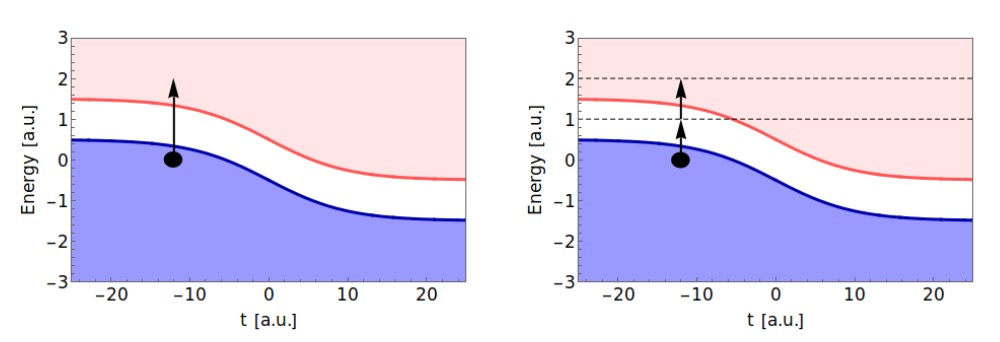
\includegraphics[width=0.8\linewidth]{figures/fig/fig1.7.jpg}
  \caption{多光子吸收示意图}
  \label{tu7}
\end{figure}

在这里,我们就不花费较长篇幅去推导多光子机制下的真空对产生率,而选择直接给出表达式:
\begin{equation}\label{ND}
 \dot N \approx \begin{cases}  \exp \left(\-\frac{\pi m^2 c^3}{e \hbar E}\right), & \gamma \ll 1 \\ (\frac{e E}{2m \omega})^{4mc^2/ (\hbar \omega)}, & \gamma \gg 1\end{cases}.
\end{equation}
其中$E$为外加电场强度,$\omega$为电场频率,$m$为电子的静止质量,$c$是光速,$\gamma$是Keldysh参数。Keldysh参数可以用来评估在对产生过程中是隧穿过程主导还是多光子吸收过程主导,定义如下:
\begin{equation}\label{Keldysh3}
 \gamma = \frac{m \omega}{e E}.
\end{equation}
此外,假设一个$n$光子吸收过程导致对产生,那么$n+m$光子过程的机会是非零的。由于$n$,$m$是任意的非负整数,这必然在相空间中产生一个明显的特征,因为产生的粒子的动量有所不同。类似于大家熟知的原子电离中的过程,我们把这种效应被称为超阈值对产生(见图\ref{tu8})。从最新的理论计算研究所知道到的,还有一种组合效应的可能性。如果电子吸收的光子能量不足以将电子推向连续体,那么还有两种可能情况。电子要么以光子的形式发射能量,重新回到狄拉克海;要么从虚态通过隧穿效应跃迁到连续体。这种动力学辅助的施温格效应的原理在图\ref{tu8}中有所说明。

\begin{figure}
  \centering
  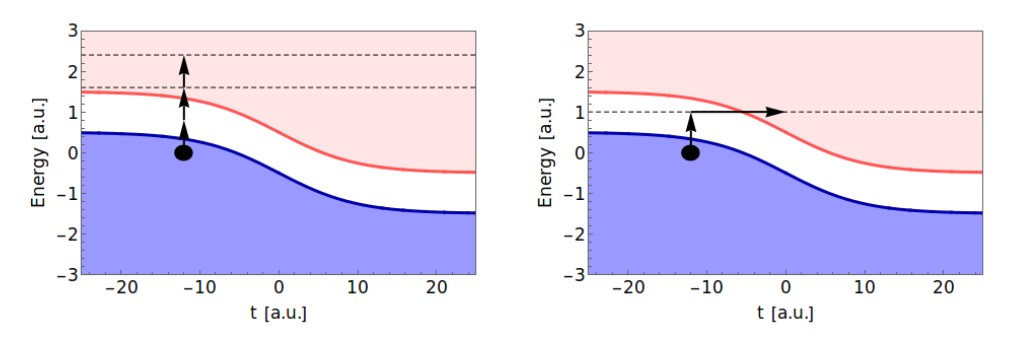
\includegraphics[width=0.8\linewidth]{figures/fig/fig1.8.jpg}
  \caption{超阈值对产生和动力学辅助的Schwinger机制示意图}
  \label{tu8}
\end{figure}

\section{研究现状}

考虑到当前激光的空间聚焦尺度远大于产生正负电子对所需的空间尺度(即电子的康普顿波长),由两束激光碰撞形成的驻波场可以被视为随时间变化的空间均匀电场。在此场下的粒子对生成问题实际上是将对产生问题推广到含时间电场的情况,研究的重点主要在于优化外部场构型以降低粒子对生成的阈值和提高对的产量,以及研究复杂强场下粒子对生成的性质。在各种复杂强外场中的真空对产生问题已经得到了广泛而深入的研究。这些复杂强外场包括由慢变强场和快变弱场组成的组合场,具有脉冲形状不对称的不同极化场,以及频率啁啾场。在这些不同配置的外场下,真空正负电子对生成过程呈现出许多新的现象,如动力学辅助下的对产生,动量谱的振荡,以及多峰干涉效应。以下给出了在不同场配置下的对生成过程中的一些重要结果,这将有助于理解本论文的主要工作。

\subsection{动力学辅助的Schwinger机制}

从公式\ref{NS}我们可以知道在弱电场下,正负粒子对的产生率呈指数级抑制,因此,用当前的激光场强度观察施温格机制对产生过程非常困难。此外,从公式\ref{ND}可以看出,多光子区域下低频激光场中的粒子对生成率也大致呈指数级抑制。因此,在目前的激光条件下仅由这两种对生成机制产生的粒子数量将非常少,于是自然而然的想到,能不能将这两种机制结合起来,来促进对的产生,我们把这结合机制叫做动力学辅助的Schwinger机制,原理可以在图\ref{tu8}右测得到一个清晰的解释。2008年Sch{\"u}tzhold等人就创造性地完成了这个工作\cite{2008d},他们的研究主要关注由强而缓慢变化的电场(施温格效应)诱导的正负电子对对从狄拉克真空中的产生,同时这个电场又被一个弱而快速变化的电磁场(动力学对产生)所叠加。在亚临界区域,这两种机制单独作用时都会被强烈抑制,但当它们联合作用时,会显著增强对生成率。强电场降低了动态粒子生成的阈值,快速的电磁场为施温格机制提供了额外的“可能”。

\subsection{脉冲形状不对称对对产生的影响}

2014年,Obulkasim等人通过量子Vlasov方程(quantum Vlasov equation, QVE) ,研究了强非对称激光电场中的电子-正电子对产生\cite{2014as}。该研究考虑了亚周期、周期和超周期激光脉冲的三种不同情况。在非对称激光脉冲场中,其中一个上升或下降侧的脉冲长度固定,而另一侧的脉冲长度改变,与对称情况相比,对产生率和数密度可以显著修改。对于这三种不同周期脉冲的每一种情况,当一侧脉冲长度恒定,另一侧脉冲长度变短(即整个脉冲被压缩)时,可以产生比相反情况(即整个脉冲被拉长)更多的对。在压缩脉冲的情况下,存在一种最优的非对称脉冲长度比,使得对数密度最大。此外,由亚周期脉冲产生的最大对数密度大于周期和/或超周期脉冲产生的对数密度。然而,在拉长脉冲的情况下,只有对于超周期激光脉冲,产生的对增强,并且也存在一种最优的非对称脉冲长度比,使得对数密度最大。另一方面,令人惊讶的是,在亚周期和周期拉长激光脉冲的两种情况下,随着脉冲的不对称性增加,对数密度单调递减。2020年,他们再使用 Dirac–Heisenberg–Wigner(DHW)方法,研究了极化电场中非对称脉冲对对产生的影响\cite{2020as}。研究探究了在三种典型的极化场:线极化,椭圆极化和圆极化场中正负电子对的生成。研究了下降脉冲长度的两种不对称性,缩短和延长。研究发现,随着脉冲长度的缩短,干涉效应消失,动量谱的峰值集中在动量空间的中心。在延长下降脉冲长度的情况下,动量谱中出现了无干涉的多环结构。研究结果显示,动量谱对脉冲的不对称性以及场的偏振非常敏感。还发现,不同偏振下的粒子的数密度对电场的不对称性敏感。对于短下降脉冲,数密度可以显著增强,超过两个数量级。

\subsection{频率啁啾对正负电子对产生的影响}

首先,我们介绍在空间均匀含时电场中频率啁啾对正负电子对产生的影响。2010年,Dumlu在啁啾激光脉冲的背景下\cite{2010c},研究已经分析了这些具有子周期结构的脉冲,并研究了啁啾参数对产生粒子的动量谱的影响。也分析了啁啾和激光脉冲的载波相位的联合效应。通过在复WKB散射方法对产生对的框架内研究势的转折点结构,定性地解释了这些效应。2013年,姜敏等人根据QVE方法,研究了频率啁啾对电子对生成的影响\cite{2013cj}。同时也考虑了周期参数,该参数表征了脉冲内激光场的周期度。在超周期和子周期激光脉冲中,频率啁啾都可以大大增强产生的对的动量分布函数和对的数密度。由超周期激光脉冲产生的对数密度大于在相同的激光频率和啁啾下由子周期脉冲产生的对数密度。对于不同的啁啾率,存在一个对应于产生的对数密度最大值的最佳周期参数。发现当周期参数低于/高于最佳值时,对数密度对啁啾率敏感/不敏感。同年,李子良等人同样运用QVE的方法研究频率变化对强脉冲激光场中真空对产生的影响\cite{2013cl}。他们发现,缓慢变化的频率可以在一定程度上影响对产生,而快速变化的频率可以在时间位于一个窄时间窗口内(在此窗口中发生频率跳跃)时,将对创建率增加几个数量级。对增强对现象背后可能的物理机制也进行了简要讨论。

2017年,Nuriman等人利用QVE方法研究了双色的频率啁啾场\cite{2017c}。他们探究了在一色和二色激光脉冲场中,通过频率啁啾产生电子对的过程。频率啁啾是指信号频率随时间的变化,在这里,它被用来调制激光脉冲。研究发现,小的频率啁啾可以沿着动量轴移动动量谱。在二色脉冲场中产生的对的数密度远高于一色脉冲场中的数密度。通过与固定频率的比较,发现频率调制对电子数量有显著的增强效应。特别是当频率较小时,适当的频率调制可以增强对产生中的多光子过程,从而促进对的产生。2019年,Obulkasim等人利用DHW方法研究在频率啁啾的不同极化电场中的对产生\cite{2019c}。他们使用实时的DHW形式来研究电场,将其模型化为具有亚临界峰值场强的均匀单脉冲场。他们计算了四种不同极化(线极化、椭圆极化、近圆椭圆极化和圆极化)以及一些线性频率啁啾的动量谱。他们发现频率啁啾导致了强烈的干涉效应和动量谱的显著变化,具体取决于所选的极化。产生的对的数密度非线性地依赖于表征极化的参数,并且对啁啾参数的变化非常敏感。对于一些研究过的频率啁啾,这可以提供三到四个数量级的数密度增强。2020年,龚弛等人使用QVE方法研究了频率调制激光场中产生的电子-正电子对的动量谱和数密度\cite{2020cg}。动量谱呈现出明显的干涉模式,这是频率调制场在动量谱上的印记,因为动量峰值对应于通过吸收不同频率组分的光子的对产生过程。此外,通过分析转折点结构,也可以定性地理解干涉效应。对数密度的研究表明,数密度对调制参数非常敏感,对于某些调制参数,可以增强2到3个数量级。2021年,王焜等人研究了对称频率啁啾效应对对产生的影响\cite{2021cw}。他们研究使用了DHW形式来研究在对称频率啁啾的电场的线、椭圆、近圆和圆极化下的电子对产生,并得到动量谱和对产量。他们发现,对于小的啁啾,极化场之间的结果差异是明显的。当啁啾参数增加时,动量谱倾向于展示由多同心环结构表征的多光子对生成。与非对称频率啁啾的情况相比,数密度的增加也非常显著。与非对称频率啁啾的情况相比,数密度的增加也非常显著。他们指出,动力学辅助的施温格机制在对称频率啁啾中增强对产生中起着重要作用。

接下来,我们再来介绍对于空间和时间都依赖的电场,我们看看频率啁啾效应如何影响对产生。2020年,Mamutjan等人研究了空间非均匀振荡电场中的啁啾效应对电子对产生的影响\cite{2020cm}.他们使用了DHW形式来研究非均匀电场下真空对产生的啁啾效应,发现对于快速振荡的电场,粒子动量谱对空间尺度和啁啾参数都敏感。对于最大的啁啾,外部场宽度的影响较小。对于慢速振荡的电场,大的空间范围内可以识别出啁啾效应,载波相位在小的空间尺度上也能显著反映出啁啾效应。在准均匀极限下,所有考虑的外部场配置都满足局部密度近似,允许人们使用来自均匀场的方法来分析非均匀场结果。2021年,Melike等人继续用DHW方法研究对称频率啁啾在不均匀电场中\cite{2021cMM}。他们研究了高频和低频模式,并考虑了两个载波包络相位。发现动量谱对啁啾敏感,导致对于不同的空间尺度以及外部场的载波相位产生不同的干涉效应。随着啁啾的增加,约化的粒子数通常会增强。也研究了场的空间尺度对减少粒子数的影响。发现在小的空间尺度上,它会增强,但在大的空间尺度上,对于考虑的场参数,它几乎不会改变。在小的空间尺度上,当应用啁啾时,约化粒子数会增强一个或两个数量级,除了余弦低频场,它只是大几倍。此外,发现通过与高频场中通常的非对称啁啾比较,对称啁啾进一步增加了约化粒子数,大约增加了两倍。同年李烈娟等人利用DHW形式来研究啁啾参数对单一场或动态辅助组合场在各种空间尺度下的约化动量谱和总粒子产量的影响\cite{2021cL}。对于单一高频场和组合场,随着啁啾的增加,动量谱的干涉效应变得更加显著。在有啁啾的动力学辅助场情况下,当两个场存在啁啾时,约化的总产量显著增强。具体来说,在动力学辅助场情况下,当应用啁啾时,小空间尺度上的减少粒子数增加了一个或两个数量级,而在大空间尺度上,它增强了大约两倍。该研究还为各种情况下的总产量和增强因子提供了一些最优的啁啾和空间尺度参数。

2023,Melike等人研究了载波包络相位对在具有对称频率啁啾的空间非均匀电场中的产生的影响\cite{2023cMM}。在高频和低频场中,他们发现由相位引起的动量谱和减少的粒子数都有周期性的变化。特别地,在低频场的情况下,这些变化更为敏感。在某些条件下,由相位引起的减少的粒子数可以增加一个数量级以上他们在动量谱中揭示了两个相关相位的一些不同类型的对称性和一个有趣的个体自对称性。相位和啁啾的联合作用在动量谱和减少的粒子数的周期性和对称性行为中提供了更灵活的参数选择,以控制和优化对产生。同年,Emin等人研究了电场啁啾对不同振荡电场中对产生的影响\cite{2023ce}。该研究主要考虑了二次和正弦啁啾电场。结果表明,啁啾显著影响了由低频隧道效应主导的电场中产生的粒子的动量谱,特别是在正弦啁啾场中,动量谱的振荡明显。然而,随着啁啾参数的增加,多光子过程逐渐显现。因此,在由多光子过程主导的高频电场中,生成粒子的数密度随着在二次啁啾场中的啁啾参数的增加而增加,而动量分布保持相对对称。在正弦啁啾电场中,引入啁啾参数立即改变了动量分布,导致对称性的破坏。此外,存在一个最优的啁啾参数,在正弦啁啾电场中,总粒子数在最优啁啾下增加了大约一个数量级以上;超过一定的阈值后,产生的粒子的数密度减少,表明在正弦电场中啁啾有抑制效应。同年,王莉等人使用计算量子场论(CQFT)研究了线性啁啾频率下复合势阱中正负电子对对增强。在适当的啁啾参数下,复合势阱下产生的电子对数量可以增加两到三倍。在低频区域,频率调制激发了干涉效应和多光子过程,这促进了电子对的生成。在高频区域,高频抑制抑制了电子对的生成。对于单个势阱,在低频区域,产生的电子对的数量可以提高几个数量级。有趣的是,胡丽娜等人还利用频率啁啾来调制相位研究了在空间非均匀电场中带有正弦相位调制的电子对产生\cite{2023ch}。重点讨论了调制参数对动量谱和各种空间尺度下的约化粒子数的影响。对于动量谱,随着调制幅度或频率的增加,干涉效应变得越来越显著,而当调制幅度时,对称性被严重破坏。对于减少的粒子数,当应用调制参数时,它会大约增加几倍,甚至一个数量级。此外,研究了空间尺度对约化粒子数的影响,发现它在小的空间尺度上迅速增加,而在大的空间尺度上趋于常数。我们还得到了可以通过不同的调制实现的最优对产生。这些结果为通过结合场的空间非均匀性和不同的相位调制选择来实现最优对产生提供了可能性。

\section{本论文的主要研究内容}
本论文采用DHW形式,对频率啁啾场下的真空正电子-负电子对问题进行了深入研究。通过对得出的结果进行详细的分析和讨论,我们进一步深化了对粒子对生成机制的理解。以下是本论文的主要工作和结构:
第2章主要介绍DHW形式。
第3章采用实时的DHW形式,研究了不对称脉冲形状在场中对电子-正电子对产生的影响进行了深入探讨,涵盖了三种不同的啁啾情况。分析了产生粒子的动量谱和数密度。
第4章研究对称频率啁啾电场对电子对产生的影响。
第5章对论文内容进行总结与展望。





